\documentclass[a4paper, 11pt]{article}


\usepackage[czech]{babel}
\usepackage[utf8]{inputenc}
\usepackage[left=2cm, top=3cm, text={17cm, 24cm}]{geometry}
\usepackage{times}
\usepackage{verbatim}
\usepackage{enumitem}
\usepackage{graphicx}
\usepackage[unicode]{hyperref}
\parskip=0.2\baselineskip % nastavuje velikost vertikální mezery mezi odstavci



\begin{document}
\begin{titlepage}
		\begin{center}
			
\includegraphics[width=0.77\linewidth]{include/FIT_logo.pdf} \\

			\vspace{\stretch{0.382}}

			\Huge{Projektová dokumentace} \\
			\LARGE{\textbf{Implementace překladače jazyka IFJ23}} \\
			\Large{Tým xhalam16, varianta TRP-izp}
			\vspace{\stretch{0.618}}
		\end{center}

		\begin{minipage}{0.4 \textwidth}
			{\Large \today}
		\end{minipage}
		\hfill
		\begin{minipage}[r]{0.6 \textwidth}
			\Large
			\begin{tabular}{l l l}
				\textbf{Marek Halamka} & \textbf{(xhalam16)} & \quad TBA,\% \\
				Šimon Motl & (xmotls00) & \quad TBA\,\% \\
				Richard Juřica & (xjuric31) & \quad TBA\,\% \\
				Jan Kroutil & (xkrout04) & \quad TBA\,\% \\
			\end{tabular}
		\end{minipage}
	\end{titlepage}

	\tableofcontents

	\newpage
	\section{Úvod}
	Překladač jazyka IFJ23 je projekt vytvořený v rámci předmětů IFJ a IAL na FIT VUT v Brně. 
	\par\noindent Cílem projektu je vytvořit překladač jazyka IFJ23, který bude překládat zdrojový kód napsaný v tomto jazyce do cílového jazyka IFJcode23 a vrací příslušný návratový kód.
	\par\noindent Program je implementován jako konzolová aplikace, která na standardní vstup přijímá zdrojový kód jazyka IFJ23 a na standardní výstup vypisuje cílový kód jazyka IFJcode23. 
	\par\noindent Překladač je implementován v jazyce C dle normy C11\footnote{ISO/IEC 9899:2011, viz. \url{https://www.iso.org/standard/57853.html}} a je rozdělen do několika modulů. Každý modul má svůj hlavičkový soubor, který obsahuje deklarace funkcí a struktur definovaných v daném modulu. 


	\section{Implementace}
	Zvolená metoda implementace je jednoprůchodový \textbf{syntaxí řízený překlad} a skládá se z částí, které jsou popsány v následujících podkapitolách.

	\subsection{Pomocné moduly a rozhraní}
	Program mimo hlavní funkce obsahuje několik důležitých modulů a rozhraní využívaných v rámci celého projektu. Jejich výčet a popis se nachází v následujících podkapitolách.
	\subsubsection{Error}
	Toto rozhraní, definované v hlavičkovém souboru \texttt{error.h}, obsahuje výčtový typ chybových stavů, které mohou nastat při běhu programu.


	\subsubsection{DynamicBuffer}
	Tento modul definovaný v souboru \texttt{dynamic\_buffer.c} má za úkol uchovávat řetězce proměnné délky.
	Korespondující hlavičkový soubor \texttt{dynamic\_buffer.h} obsahuje deklarace funkcí a struktur definovaných v tomto modulu.
	\par\noindent Rozhraní obsahuje strukturu \texttt{dynamic\_buffer}, která obsahuje \textbf{ukazatel} na alokovanou paměť, \textbf{kapacitu} alokované paměti a \textbf{velikost} obsazené paměti.
	\par\noindent Modul obsahuje funkce pro inicializaci, uvolnění, realokaci a práci s řetězci. Buffer se v případě naplění automaticky realokuje na dvojnásobek své původní kapacity.
	\par\noindent Pomocí výše zmíněných funkcí jsme definovali abstraktní datový typ \texttt{DynamicBuffer}, který je využíván v dalších částech projektu.

	\newpage
	\subsubsection{Token}
	Hlavičkový soubor \texttt{token.h} obsahuje definici struktury \texttt{token}, která reprezentuje token.
	\par\noindent Struktura obsahuje typ tokenu, hodnotu tokenu a textovou reprezentaci tokenu ve zdrojovém souboru. 
	\par\noindent \textbf{Typ tokenu} je definován výčtovým typem \texttt{token\_type}, který obsahuje všechny typy tokenů jazyka IFJ23. 
	\par\noindent \textbf{Hodnota tokenu} je typu \texttt{union}, a nabývá buď hodnoty odpovídající číslené hodnotě tokenu, nebo ukazatele na dříve definovanou strukturu \texttt{DynamicBuffer}, která reprezentuje řetězec.
	Typ union byl zvolen z důvodu úspory paměti, protože token může obsahovat pouze jednu z těchto hodnot.
	\par\noindent \textbf{Textová reprezentace tokenu} ve zdrojovém souboru je uložena jako ukazatel na strukturu \texttt{DynamicBuffer}, který obsahuje řetězec.
	Je uchovávána z důvodu implementace funkce \texttt{peek\_token}, která je podrobněji popsána v sekci \ref{sec:lex}.

	\subsubsection{Tabulka symbolů}
	Tabulka symbolů slouží k uložení informací o proměnných a funkcích.
	\par\noindent Deklarace proměnné či funkce odpovídá vytvoření záznamu v tabulce symbolů, kde klíčem je \textbf{identifikátor} proměnné.
	\par\noindent Dle zvolené varianty zadání je tabulka symbolů implementována jako \textbf{TRP s otevřenou adresací}.
	\par\noindent Implicitní rozptýlení využívá \textbf{lineární} určení kroku při výpočtu dalšího volného indexu. 
	\par\noindent Tabulka symbolů je implementována v souboru \texttt{symtable.c} s rozhraním v souboru \texttt{symtable.h}.
	\par\noindent Rozhraní obsahuje funkce pro inicializaci, uvolnění, vložení a vyhledání položky v tabulce symbolů či vytvoření nové položky.
	\par\noindent Kromě těchto funkcí obsahuje i signaturní \textbf{hashovací funkci}, která je použita při transformaci klíče, na index do tabulky symbolů.
	\begin{figure}[h]
		\centering
		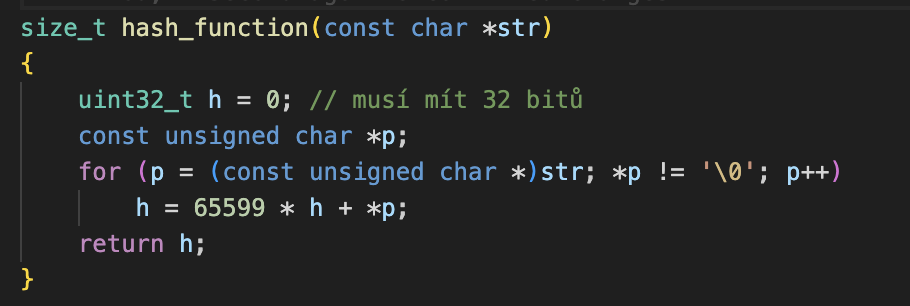
\includegraphics[width=0.5\linewidth]{include/hash_function.png}
		\caption{Hashovací funkce}
		\label{fig:hash_function}
	\end{figure}

	\par\noindent Při vytváření hashovací funkce jsme čerpali informace z předmětů IJC, IAL a zde: citace.


	\par\noindent Tabulka se v případě naplnění automaticky \textbf{realokuje} na dvojnásobek své původní kapacity.
	\par\noindent V programu rozlišujeme mezi \texttt{GLOBÁLNÍ} a \texttt{LOKÁLNÍ} tabulkou symbolů. Globální tabulka symbolů je vytvořena při inicializaci programu a je uvolněna při jeho ukončení. Lokální tabulka symbolů je vytvořena při vstupu do bloku a je uvolněna při jeho opuštění.
	\par\noindent Tyto typy tabulek se liší mimojiné i v datech, které uchovávají. Funkce pro práci s tabulkou symbolů jsou implementovány tak, aby bylo možné používat stejné funkce pro oba typy tabulek. Docíleno je to pomocí ukazatele typu \texttt{void}, který je přetypován na konkrétní typ tabulky symbolů v závislosti na tom, zda se jedná o \texttt{GLOBÁLNÍ} nebo \texttt{LOKÁLNÍ} tabulku symbolů.
	


	\subsubsection{Parameter list}
	Parametry funkcí jsou uchovávány v seznamu, který je implementován jako \textbf{jednosměrně vázaný seznam}.
	\par\noindent Seznam je implementován v souboru \texttt{symtable.c} s rozhraním v souboru \texttt{symtable.h}.
	\par\noindent Rozhraní obsahuje funkce pro inicializaci, uvolnění, vložení a vyhledání položky v seznamu.
	\par\noindent Implementací výše zmíněných funkcí je definován abstraktní datový typ \texttt{parameter\_list\_t}, který je vy\-užíván v dalších částech projektu.


	\subsubsection{Stack}
	Zásobník je v projektu využíván na více místech, pokaždé pro ukládání jiného typu dat.
	\par\noindent Proto byl zásobník implementován jako \textbf{obecný zásobník}, který je definován v souboru \texttt{stack.c} s rozhraním v souboru \texttt{stack.h}.
	\par\noindent Zásobník uchovává položky typu \texttt{Stack\_Frame}, které obsahují ukazatel na data typu \texttt{void}. Tím je umožněno ukládat na zásobník jakýkoliv typ dat.
	\par\noindent Rozhraní obsahuje známé funkce pro práci se zásobníkem. Tím je definován abstraktní datový typ \texttt{Stack}.
	\par\noindent Za účelem ulehčení řešení některých problémů, které se vyskytly při implementaci, rozhraní zásobníku poskytuje i funkci \texttt{Stack\_get(stack,index)}, která vrací položku na zadaném indexu.
	\par\noindent Jelikož struktura ukládá data jako ukazatel, je potřeba dát pozor, nad čím voláme operaci \texttt{free}. Proto byla implementována funkce \texttt{stack\_empty}, která uvolní všechny ukazatele na zásobníku. Funkce předpokládá, že na zásobníku jsou pouze ukazatele na dynamicky alokovanou paměť.
	\par\noindent Pokud dojde k naplnění zásobníku, je automaticky \textbf{realokován} na dvojnásobek své původní kapacity.

	\subsection{Lexikální analýza} \label{sec:lex}
	Lexikální analýza je definována v souboru \texttt{scanner.c} s rozhraním v souboru \texttt{scanner.h} a implementována jako \textbf{deterministický konečný automat}. Graf konečného automatu je zobrazen na obrázku ODKAZ.
	\par\noindent Automat se rozhoduje na základě aktuálního stavu a načteného znaku ze vstupního souboru.
	\par\noindent V jazyce C je implementován pomocí konstrukce \texttt{if...else if}, kde každá větev odpovídá jednomu stavu automatu. Automat také využívá a nastavuje pomocné statické globální proměnné, které jsou definovány v souboru \texttt{scanner.h}. 


	
	\subsection{Syntaktická analýza}

	\subsection{Sémantická analýza}

	\subsection{Generování cílového kódu}








    

\end{document}